\subsection{Архитектура платформы}
\label{sec:fw_arch}

В этом разделе будет рассмотрена укрупненная схема архитектуры платформы; расположение и назначение компонентов системы и их взаимодействие.

После определения спектра глобальных задач, подлежащих решению в рамках реализации платформы, и выбора используемых для их решения технологий, инструментов и подходов, а также учитывая опыт существующих разработок, направленных на решение поставленной задачи, в особенности {\it VBA} и {\it VSTA}, была разработана концептуальная модель взаимодействия основных компонентов платформы~\cite{patterns-of-enterprise-app}.

Как видно на рисунке \ref{fw_arch1}, система состоит из двух отдельных процессов. Такая архитектура обусловлена необходимостью поддержку отладки расширений, а отладчик, как известно, должен выполняться в отдельном процессе. Кроме того, хост-процесс IDE является дочерним для процесса хост-приложения. Управление этими процессами организовано таким образом, что в случае прекращения из-за критической ошибки работы процесса, обслуживающего IDE, этот процесс будет автоматически перезапущен. В таком случае система продолжит работу в штатном режиме. Напротив, при сбое в процессе хост-приложения, будет остановлен так же хост-процесс IDE, что позволяет предотвратить возникновения в системе <<паразитных>> процессов.

Согласно разделу \ref{sec:ide-integration}, в качестве внешней среду разработки была выбрана свободная среда разработки с открытым исходным кодом SharpDevelop. Более того, благодаря совместимости библиотек входящих в состав этой IDE, реализована поддержка версий SharpDevelop 3.2 и 4.1, а так же не исключается возможность поддержки последующих версий. Таким образом, реализуемая платформа может быть с успехом использована в приложениях, реализованных на различных версиях платформы .NET.

\begin{figure}[!h]
    \centering
    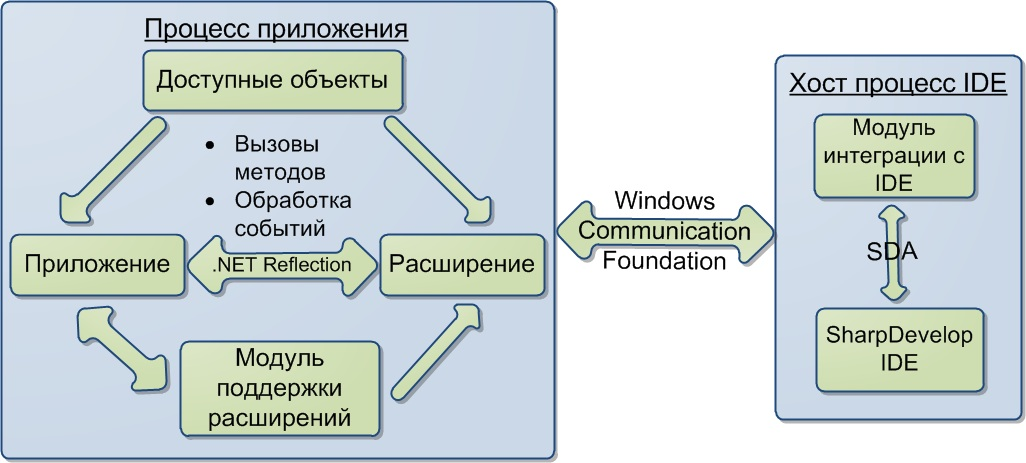
\includegraphics[width=15cm]{fw_arch1.jpg}
    \caption{Взаимодействие компонентов системы}
    \label{fw_arch1}
\end{figure}

Межпроцессное взаимодействие в разрабатываемой системе было решено реализовать при помощи именованных каналов {\tt (named pipe)} из библиотеки WCF (Windows Communication Foundation)~\cite{wcf-services}. Выбор WCF обусловлен тем, что эта библиотека входит в состав .NET Framework, и использование ее будет наиболее оправдано для разработки приложения под эту платформу. Реализация именнованых каналов в WCF --- NetNamedPipe, выбрана по причине того, что в рамках решения задачи по обеспечению взаимодействия двух процессов на локальной машине нет необходимости в использовании более сложных и емких механизмов взаимодействия, чем именованные каналы. Подробнее особенности реализации межпроцессного взаимодействия были рассмотрены ранее в разделе~\ref{sec:ipc}.

Взаимодействие между процессами происходит по двум отдельным именованным каналам, так как инициировать запросы (то есть выступать в роли сервера) могут оба процесса, и механизм <<запрос --- ответ>> в данном случае не подходит.

Более того, адреса, по которым взаимодействуют процессы выбираются случайно, что позволяет без возникновения конфликтов запускать множество пар процессов <<приложение --- IDE>>. Такое решение позволит использовать разрабатываемую платформу в нескольких приложениях одновременно.

Для работы с расширениями и IDE в приложение должен быть интегрирован специальный модуль, выполняющий сервисные задачи по обеспечению взаимодействия расширения с приложением, приложения с хост-процессом IDE, а так же предоставляющий пользователю набор визуальных компонент для управления системой. Этот модуль показан на рисунке \ref{fw_arch1} (Модуль поддержки расширений). Его назначение и особенности разработки будут описаны далее.

Взаимодействие расширения и приложения реализовано через {\it .NET Reflection}~\cite{cs2008-dotnet35}, как описано в разделе~\ref{sec:extention_interaction}. Взаимодействие осуществляется через динамическое привязывание к доступным объектам приложения, которые должны подчиняться определенным <<правилам игры>>, чтобы быть доступными для расширения. Выделение видимых объектов и создание уровня доступа к ним --- главная задача интеграции платформы в готовое приложение. Подробнее особенности интеграции разрабатываемой платформы были рассмотрены в разделе~\ref{sec:app-integration}.